%%%%%%%%%%%%%
%  Ch1 : Generalities  %
%%%%%%%%%%%%%

\chapter{Aerodynamic Force}
\section{Derivation of the conservation laws}
	\subsection{Mass conservation}
		
		\begin{wrapfigure}[9]{l}{7.5cm}
		\vspace{-5mm}
		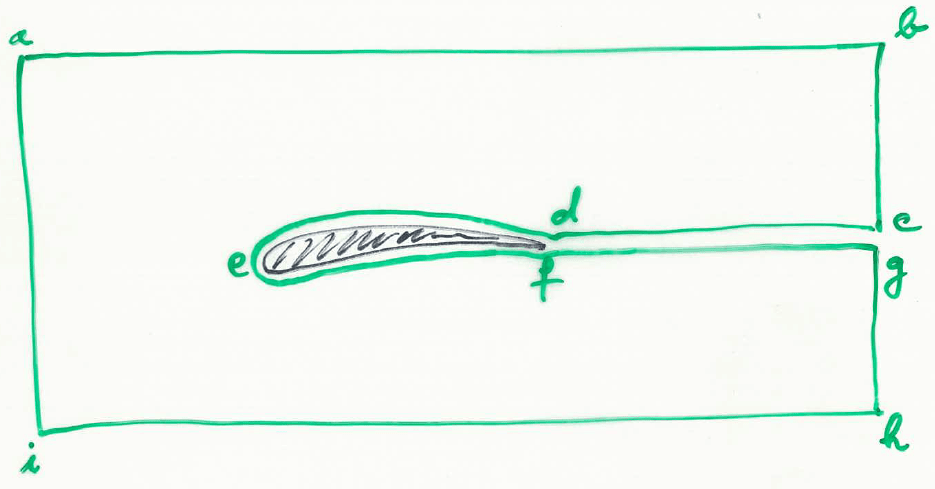
\includegraphics[scale=0.3]{ch1/1}
		\captionof{figure}{}
		\end{wrapfigure}
		Consider the closed control volume S* (abhi) around the airfoil. It is a 2D view, but imagine that we have a 3D configuration with Z axis perpendicular to the sheet. Be aware that the normal is always perpendicular to the contour and is external! The fundamental integral form of the mass conservation equation is:\\
		
		\begin{equation}
		\frac{d}{dt}\int _V \rho \, dV + \oint _S \rho \vec{v} \, d\vec{S} = 0.
		\end{equation}

		By applying Gauss theorem $\oint _S \vec{a}.\vec{n}\, dS = \int _V \nabla\vec{a}\, dV$, and regrouping the term in a unique integral, we obtain:
		
		\begin{equation}
		\int _V \left[\frac{d \rho}{d t} + \nabla .(\rho \vec{v})\right]\, dV = 0. 
		\end{equation}
		
		Considering this to be true for all volumes, the integral disappear and gives the 
		
		\begin{center}
		\theor{
		\textbf{Continuity equation}
		\begin{equation}
		\frac{d \rho}{d t} + \nabla .(\rho \vec{u}) = 0
		\label{eq:1.3}
		\end{equation}
		}		
		\end{center}
		
		Another form can be found by introducing the material derivative $\dot{\rho} = \frac{d\rho}{dt} + (\vec{v}.\nabla )\rho$, and if we are in a steady state, the time derivative goes away. 
		
	\subsection{Momentum equation}
		The general form of the momentum equation is: 
		
		\begin{equation}
		\rho \dot{\vec{v}} = \frac{\D \rho \vec{v}}{\D t} + \rho (\vec{v}\nabla ) \vec{v} = -\nabla p + \nabla \bar{\bar{\tau}}.
		\end{equation}
		
		By considering a steady state, the time derivative goes away. If we consider the x component of the velocity, we can expend the derivative to the whole left term as:
		
		\begin{equation}
		\rho (\vec{v}\nabla ) v_x = \nabla (\rho \vec{v} v_x) - v_x \cancel{\nabla (\rho \vec{v})}
		\label{eq:1.5}
		\end{equation}
		
		where the last term is null related to \eqref{eq:1.3} in steady state. Integrating both sides around the volume contained in the closed surface S (abcdefghi on figure) in \eqref{eq:1.5}, and applying Gauss theorem, we obtain:
		
		\begin{equation}
		\oint _{S} \vec{v} (\rho \vec{v} \vec{n}) \, dS = -\oint _{S} p \, d\vec{S} + \oint _{S} \bar{\bar{\tau}} \, d\vec{S}.
		\label{eq:1.6}
		\end{equation}		 
		
		Let's now apply this equation to the new closed contour $S* = S - \mbox{airfoil} - cd - fg$ (previous abhi in fact). \eqref{eq:1.6} becomes:
		
		\begin{equation}
		\begin{aligned}
		&\oint _{S^*} \vec{v} (\rho \vec{v} \, d\vec{S})  + \cancel{\oint _{\mbox{airfoil}} \vec{v} (\rho \vec{v} \, d\vec{S})} + \cancel{\oint _{cd+fg} \vec{v} (\rho \vec{v} \, d\vec{S})} 
		\\&= -\oint _{S^*} p \, d\vec{S} -\oint _{\mbox{airfoil}} p \, d\vec{S}-\cancel{\oint _{cd + fg} p \, d\vec{S}}+ \oint _{S^*} \bar{\bar{\tau}} \, d\vec{S} +\oint _{\mbox{airfoil}} \bar{\bar{\tau}}\, d\vec{S} +\cancel{\oint _{cd + fg} \bar{\bar{\tau}}\, d\vec{S}}
		\end{aligned}
		\label{eq:1.7}
		\end{equation}
		
		where the $cd + fg$ components cancels each other if we consider that they are infinitely close to each other, as they are opposite. The airfoil integral in the left hand side is null because the wing can not be penetrated by the flow. If we manipulate the equation to refind the \eqref{eq:1.6} shape by regrouping airfoil terms in an additional $\vec{R}$ term. Taking account the orientation of normals, the signs will be chosen in the way $\vec{R}$ is a
		
		\begin{center}
		\theor{
		\textbf{Force applied on the wing}
		\begin{equation}
		\vec{R} = \oint _{\mbox{airfoil}} p\, d\vec{S} - \oint _{\mbox{airfoil}} \bar{\bar{\tau}}\, d\vec{S}	
		\end{equation}
		}
		\end{center}
		
		so that \eqref{eq:1.7} becomes, after considering S* to be a contour in the \textbf{far field} so that viscous effects vanish (to avoid other parameters calculation):
		
		\begin{equation}
		\oint _{S^*} \vec{v} (\rho \vec{v} \, d\vec{S}) = -\oint _{S^*} p \, d\vec{S} + \cancel{\oint _{S^*} \bar{\bar{\tau}} \, d\vec{S}} - \vec{R}.
		\label{eq:1.9}
		\end{equation}
		
		We still have to measure the pressure.
		
		\subsubsection{Uniform p along S*}
				\begin{wrapfigure}[11]{l}{6.5cm}
				\vspace{-5mm}
				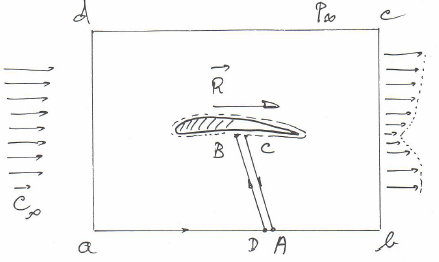
\includegraphics[scale=0.52]{ch1/2}
				\captionof{figure}{}
				\end{wrapfigure}
				By considering this (assumption of far field), we can compute the force only by knowing the far field parameters. Indeed, uniform pressure implies null surface integral, so that \eqref{eq:1.9} becomes:
				
				\begin{equation}
				\vec{R} = -\oint _{S^*} \vec{v} (\rho \vec{v} \, d\vec{S}).
				\end{equation}
				
				The velocity term remains, as by experience we know that there is a \textbf{wake} making the velocity profile non-uniform. Let's now consider that the velocity is horizontal so that $\vec{R} = R.\vec{1}_x$, at the inlet we have $\vec{v}$ and $\vec{n}$ are opposed while at the outlet they are in the same direction: 
				
				\begin{equation}
				\vec{R} = \int _a^d \vec{v}\, d\dot{m} - \int _b^e \vec{v}\, d\dot{m} > 0
				\end{equation}
				
				showing that there is only \textbf{drag} force.
				
		\section{The aerodynamic lift}
			We know in practice that there is also a lift force. In fact, the assumption of uniform pressure is wrong because the pressure effects induced by the body remains at a long distance from the body. We have to analyse the \textbf{non uniform} p along S*. In order to apply Bernouilli equation $p + \frac{1}{2}\rho v^2 = cst$, let's add the constants $p_\infty$ and $v_\infty$ to \eqref{eq:1.9}, as $\oint p_\infty\, d\vec{S} = p_\infty \oint d\vec{s} = 0$: 
			
			\begin{equation}
				\vec{R} = -\oint _{S^*} (p-p_\infty) \, d\vec{S} - \oint _{S^*} (\vec{v}-\vec{v}_\infty) \, d\dot{m}
				\label{eq:1.12}
			\end{equation}
			
			Let's express $\vec{v} = \vec{v}_\infty + \vec{\delta _c}$ with $\vec{\delta _c}$ a perturbation. Introducing this in Bernouilli equation: 
			
			\begin{equation}
			\begin{aligned}
			p_\infty +\frac{1}{2} \rho \cancel{\vec{v}_\infty ^2} = p + \frac{1}{2} \rho( &\vec{v}_\infty + \vec{\delta _c})^2 = p + \frac{1}{2} \rho (\cancel{\vec{v}_\infty ^2} + 2 \vec{v}_\infty \vec{\delta _c} + \cancel{\vec{\delta _c}^2}) \\
			&\Rightarrow p-p_\infty = - \rho\vec{v}_\infty \vec{\delta _c}	.		
			\end{aligned}
			\end{equation}
			
			If we replace this result in \eqref{eq:1.12}, we find:
			
			\begin{equation}
			\begin{aligned}
			\vec{R} &= \oint _{S^*} \rho (\vec{v}_\infty \vec{\delta _c} ) \, d\vec{S} - \oint _{S^*} \rho \vec{\delta _c} [(\vec{v}_\infty + \cancel{\vec{\delta _c}} ) \, d\vec{S}] \\
			&=\oint _{S^*} \rho [(\vec{v}_\infty \vec{\delta _c}) \, d\vec{S} - \vec{\delta _c} [(\vec{v}_\infty . d\vec{S})]
			\end{aligned}
			\end{equation}
			
			by using a vector property $\vec{a} \times (\vec{b} \times \vec{c}) = (\vec{a} \vec{b})\vec{c} - (\vec{a}\vec{c})\vec{b}$:
			
			\begin{equation}
			= \rho \vec{v}_\infty \times \oint _{S^*} \vec{\delta _c} \times d\vec{S} = \rho \vec{v}_\infty \times \left[\oint _{S^*} \vec{v} \times d\vec{S} - \cancel{\oint _{S^*} \vec{v}_\infty \times d\vec{S}}\right]
			\end{equation}
			
			and by applying Stokes theorem $\oint _S \vec{a} \times d\vec{S} = \int _V \nabla \times \vec{a} \, dV$:
			
			\begin{equation}
			= \rho \vec{v}_\infty \times \int  (\nabla \times \vec{v})\, dV = \rho \vec{v}_\infty \times \int  \vec{\omega}\, dV
			\end{equation}
			
			where $\vec{w}$ is the \textbf{vorticity vector} of direction $\vec{1}_z$ (pointing in the paper):
			
			\begin{equation}
			\vec{\omega} = 
			\left| \begin{array}{ccc}
			\vec{1}_x & \vec{1}_y & \vec{1}_z \\ 
			\D _x & \D _y & 0 \\ 
			v_x & v_y & 0
			\end{array} 
			\right| 
			= [\D _x v_y - \D _y v_x] \vec{1}_z
			\end{equation}
			
			This shows that the lift force is always perpendicular to the flow!
		
	\section{The Kutta-Joukowski formula}
		We will now introduce the circulation $\Gamma = - \oint \vec{v} \, d\vec{l} >0$   around a body. The convention is to take the anticlockwise direction for $d\vec{l}$ and so for $\Gamma$ to be $>0$ we must have $\vec{v}$ in the clockwise direction. There is a link between the lift force and the circulation. Let's introduce \textbf{Stokes theorem}:
		
		\begin{equation}
			\oint \vec{a} d\vec{l} = \int _S (\nabla \times \vec{a})\, d\vec{S} \qquad \Rightarrow -\Gamma = \int _S \vec{\omega} d\vec{S}.
		\end{equation}
		
		We remember that:
		\begin{equation}
		\begin{aligned}
		\vec{R} &= \rho \vec{v}_\infty \times \int  \vec{\omega}\, dV = \rho \vec{v}_\infty \times \int  l\vec{\omega}\, dS \qquad \Leftrightarrow \frac{\vec{R}}{l} = \rho \vec{v}_\infty \times \int  \vec{\omega}\, dS \\
		\frac{\vec{R}}{l}&= \rho \vec{v}_\infty \times \int  \vec{\omega}\, (d\vec{S}.\vec{1}_z) = \rho \vec{v}_\infty \times (-\Gamma)\vec{1}_z = \rho v_\infty \Gamma \,\vec{1}_y
		\end{aligned}
		\end{equation}
		
		to finally obtain a very good approximation of the lift:
		
		\begin{center}
		\theor{
		\textbf{Kutta formula for lift 2D airfoil}
		\begin{equation}
		|R| = \rho v_\infty \Gamma 
		\end{equation}
		}
		\end{center}
		
	\subsubsection{Application to airfoils}
		\begin{wrapfigure}[8]{l}{6.5cm}
		\vspace{-5mm}
		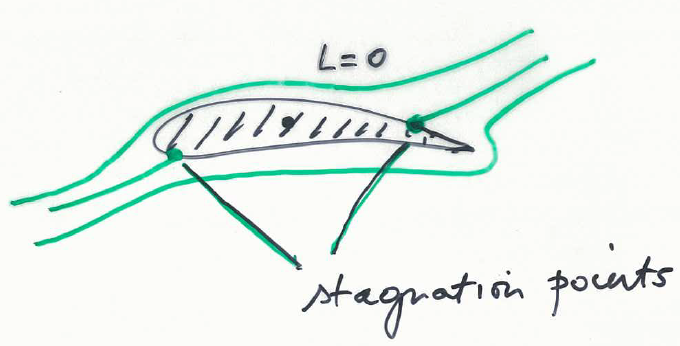
\includegraphics[scale=0.35]{ch1/3}
		\captionof{figure}{}
		\end{wrapfigure}
		In inviscid case, the Kelvin theorem states that there cannot be vorticity, so no lift. If we take an arbitrary contour around the airfoil we will have no circultion. In inviscid case we can never get a lift $\rightarrow$ D’alembert paradox. At the trailing edge, if the flow wants to continue on the other corner from below, the velocity must be infinity so that the flow separates. But this is not the case in reality. \\

		\begin{wrapfigure}[7]{r}{6.5cm}
		\vspace{-5mm}
		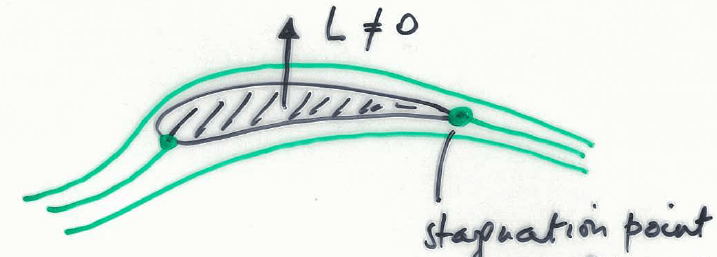
\includegraphics[scale=0.35]{ch1/4}
		\captionof{figure}{}
		\end{wrapfigure}
		After some processes we can obtain the stagnation point on the trailing edge so that we satisfy the Kutta condition (the flow has to leave the airfoil smoothly). So in this case, there is a circulation if we take a contour that contains the airfoil, but for all contour that does not contain the airfoil it is null. But why to put the stagnation point at the trailing edge? This is purely physics. $\Gamma$ varies with the stagnation point position, but only one corresponds to the Kutta condition. \\
		
		\begin{wrapfigure}[16]{l}{4cm}
		\vspace{-5mm}
		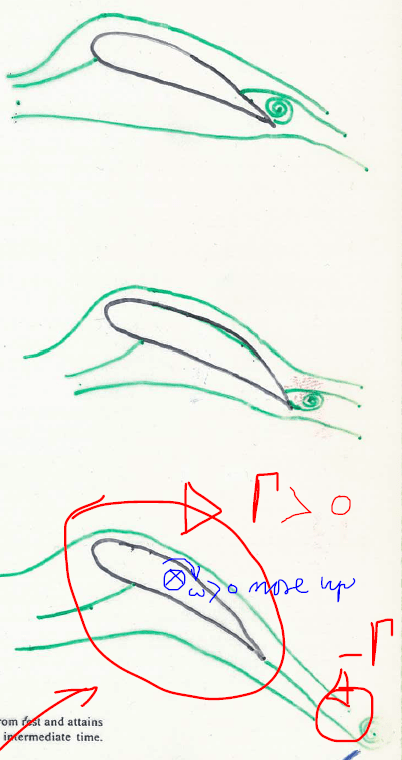
\includegraphics[scale=0.35]{ch1/5}
		\captionof{figure}{}
		\end{wrapfigure}
		What happens is that initially we have the first kind of flow, then the formation of the starting vortex due to viscous effects (separation) which is compensated by a \textbf{bound vortex} around the airfoil (to respect Kelvin theorem of irrotational flow) that makes $\Gamma \neq 0$. Then the vortex goes away to infinity. Indeed if we take $R = \rho v_\infty \Gamma$, $\Gamma \neq 0$, so we have lift. 
		
		We can show that every contour containing the airfoil has a non 0 circulation. Let's proof that a contour that doesn't contain the airfowl has $\Gamma =0$: 
		
		ADD FIGURE (1)
		
		\begin{equation}
		\oint _{C} \vec{v}\, d\vec{l} = \oint _{\mbox{airfoil}} \vec{v}\, d\vec{l} + \oint _{cd} \vec{v}\, d\vec{l} + \oint _{fg} \vec{v}\, d\vec{l} = 0. 
		\end{equation}
		
		As the contour elements are exactly opposed to each other, the result is null. 